\documentclass[a4paper,11pt, footsepline]{book}
\usepackage[T1]{fontenc}
\usepackage[utf8]{inputenc}
\usepackage{lmodern}
\usepackage{textcomp}

\usepackage{hyperref}
\usepackage{graphicx}
\usepackage[english]{babel}

\usepackage{graphicx}
\usepackage{amsmath}
\usepackage{nameref}
\usepackage{hyperref}
\usepackage[linesnumbered, boxed]{algorithm2e}
\usepackage[automark,footsepline,plainfootsepline,headsepline]{scrpage2}
\usepackage{listings, newtxtt}
\lstset{basicstyle=\ttfamily, keywordstyle=\bfseries}

\SetAlCapSkip{1em}


\renewcommand*{\algorithmcfname}{Code listing}
\renewcommand*{\algorithmautorefname}{Code listing}
\SetKwInput{KwInput}{Input}
\SetKwInput{KwOutput}{Output}
\SetKwProg{Fn}{def}{:}{}
%\newcommand\mycommfont[1]{\footnotesize\ttfamily\textcolor{blue}{#1}}
%\SetCommentSty{mycommfont}
\SetStartEndCondition{ }{}{}%
\SetKwComment{Comment}{$\triangleright$\ }{}
\SetKwFunction{Range}{range}%%
\SetKw{KwTo}{in}
\SetKwFor{For}{for}{\string:}{}%
%\renewcommand{\forcond}{$i$ \KwTo\Range{$n$}}
\AlgoDontDisplayBlockMarkers\SetAlgoNoEnd\SetAlgoNoLine%

\usepackage[printonlyused]{acronym}

\newcommand*{\fullref}[1]{\hyperref[{#1}]{\autoref*{#1} \nameref*{#1}}} % One single link
\renewcommand*\footnoterule{}

\makeatletter
\renewcommand{\@chapapp}{}% Not necessary...
\newenvironment{chapquote}[2][2em]
  {\setlength{\@tempdima}{#1}%
   \def\chapquote@author{#2}%
   \parshape 1 \@tempdima \dimexpr\textwidth-2\@tempdima\relax%
   \itshape}
  {\par\normalfont\hfill--\ \chapquote@author\hspace*{\@tempdima}\par\bigskip}
\makeatother




% Book's title and subtitle
\title{\Huge \textbf{High Performance Computing with Python} \vspace{4mm} \\ \huge Final Report}
% Author
% \author{\textsc{First-name Last-name}\footnote{email address}}
\author{\textsc{Name} \\ \vspace{3mm}\text{matricular number}  \\
\vspace{3mm}\text{mail}}


\begin{document}

\makeatletter
    \begin{titlepage}
        \begin{center}
            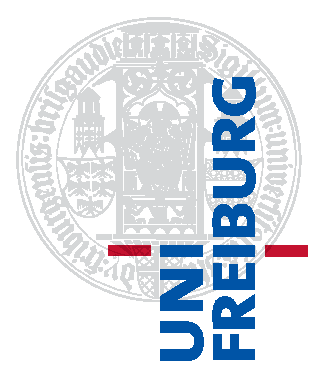
\includegraphics[width=0.5\linewidth]{logos/Uni_Logo-Grundversion_E1_A4_CMYK.eps}\\[4ex]
            {\huge \bfseries  \@title }\\[2ex] 
            {\LARGE  \@author}\\[30ex] 
            {\large \@date}
        \end{center}
    \end{titlepage}
\makeatother
\thispagestyle{empty}
\newpage



\tableofcontents

\begin{acronym}
\section*{Abbreviations}
\acro{bte}[BTE]{Boltzmann Transport Equation}
\acro{ci}[CI]{Continuous Integration}
\acro{lbm}[LBM]{Lattice Boltzmann Method}
\acro{simd}[SIMD]{Single Instruction Multiple Data}
\acro{mpi}[MPI]{Message Passing Interface}
\end{acronym}
\mainmatter

\chapter{Introduction}
The \acf{lbm} is a numerical, parallelizable and efficient scheme for simulating fluid flows based on the discretization of (continuous) \acf{bte}.\cite{McNamara.1988} In addition, the \ac{lbm} can be extended with boundary conditions. The key property of the \ac{lbm} is that it is a discrete kinetic theory approach featuring a mescoscale description of the microstructure of the fluid instead of discretizing macroscopic continuum equations. Other key advantages of the \ac{lbm} include: efficient implementation by parallelization and the \ac{lbm} can be applied to different kind of lattices.

We show in several two-dimensional (i.e. planar) test cases, i.e. \textit{Couette flow}, \textit{Poiseuille flow} and \textit{Von K\'{a}rm\'{a}n's vortex street}, the correctness of our implementation as well as the significant reduction of computational time of the von K\'{a}rm\'{a}n's vortex street simulation by means of parallelization by spatial domain decomposition using \textit{Python} as programming language with its highly efficient \textit{numpy} library \cite{Oliphant.2006,vanderWalt.2011} and the \acf{mpi} \cite{Dalcin.2005, Dalcin.2008, Dalcin.2011}.

All code is available at \url{https://github.com/infomon/lattice_boltzman_parallel_solver} under BSD license. We give the instructions how to reproduce the results of the experiments conducted in this report in the \textit{README}.

\section*{Structure of report}
The remainder of the report is organized as follows:
\begin{itemize}
\item \textbf{Chapter \ref{ch-method}} describes the \ac{lbm}. More specifically, we describe how we discretize the \textit{\acf{bte}} resulting in the \ac{lbm}. We also show how macroscopic quantities, e.g. density and velocity, can be calculated from the microscopic simulation. In addition, we describe several boundary conditions that can be applied in the \ac{lbm}.
\item \textbf{Chapter \ref{ch-implementation}} describes how the \ac{lbm} is implemented using \textit{Python} as programming language. We also show how we parallelized the implementation and how we ensured software quality by unit testing.
\item \textbf{Chapter \ref{ch-results}} conducts extensive experiments showing the applicability and correctness of the implementation of the solver for the \ac{lbm}. 
\item \textbf{Chapter \ref{ch-conclusion}} concludes this report.
\end{itemize}
\chapter{Lattice Boltzmann Method}\label{ch-method}
\section{Overview}
In this chapter we describe the \acf{lbm}. The main idea of the \ac{lbm} is to \textit{simulate a fluid density statistically on a lattice} instead of solving (and also discretizing) the Navier-Stokes equations.
\section{Boltzmann Transport Equation}\label{sec-bte}
The \acf{bte} $\frac{df}{dt}$ defines the fundamental differential equation of kinematic gas theory. It describes the evolution of the probability density function $f_(\mathbf{r},\mathbf{v},t)$ for finding a molecule with mass $m$ and velocity $\mathbf{v}$ at position $\mathbf{r}$ over time $t$. Huang \cite{Huang.1987} shows that the \ac{bte} relaxes to the Maxwell velociy distribution function. Bhatnagar et al. \cite{Bhatnagar.1954} approximate the relaxation of $f$ towards $f^{eq}$ as follows:
\begin{equation}
\label{eq-bte}
\frac{df(\mathbf{r},\mathbf{v},t)}{dt}=-\frac{f(\mathbf{r},\mathbf{v},t)-f^{eq}(\mathbf{v};\rho(\mathbf{r,t}),\mathbf{u}(\mathbf{r},t),T(\mathbf{x},t))}{\tau}
\end{equation}
where $\tau$ is the so-called characteristic time, $\rho$ is the mass density, $u$ is the average velocity at position $\mathbf{x}$ and $T$ is the temperature (see section \ref{sec-momentUpdate} for more details). The characteristic time determines how fast the fluid converges towards the equilibrium depending on the viscosity of the fluid. The higher the viscosity, the slower it converges towards the equilibrium. Note, that eq. \ref{eq-bte} satisfies the Navier-Stokes equations.
\subsection*{Discretization of the \ac{bte}}
The \ac{bte} of eq. \ref{eq-bte} is defined in the continuous domain. In order to work with the \ac{bte} on the computer we have to discretize it in space, velocity and time. The space discretization can be done by just using a discrete lattice (e.g. two-dimensional array). To discretize the velocity and time we have to impose that the velocity multiplied with the time is equal to some integer, i.e. the particle can only travel on the given lattice and not in-between lattice nodes. 

We discretize the velocity directions with the D2Q9 scheme (see fig. \ref{fig:mesh}a), which is two-dimensional and consists of nine discrete velocity directions. The velocity directions point to each of its neighbors in the Moore neighborhood. Note, that at the central lattice node the particle is at rest. We define the velocity vectors as follows:
\begin{equation}
\mathbf{c_i}=\begin{pmatrix}
0 & 1 & 0 & -1 & 0 & 1 & -1 & -1 & 1\\
0 & 0 & 1 & 0 & -1 & 1 & 1 & -1 & -1
\end{pmatrix}.
\end{equation}
Therefore, we discretize the probability density function $f(\mathbf{r},\mathbf{v},t)$ to obtain the discrete probability density function $f_{i}(\mathbf{x},t)$, where the subscript $i$ indicates the direction and $\mathbf{x}$ is the discrete lattice.
\begin{figure}
  \begin{center}
   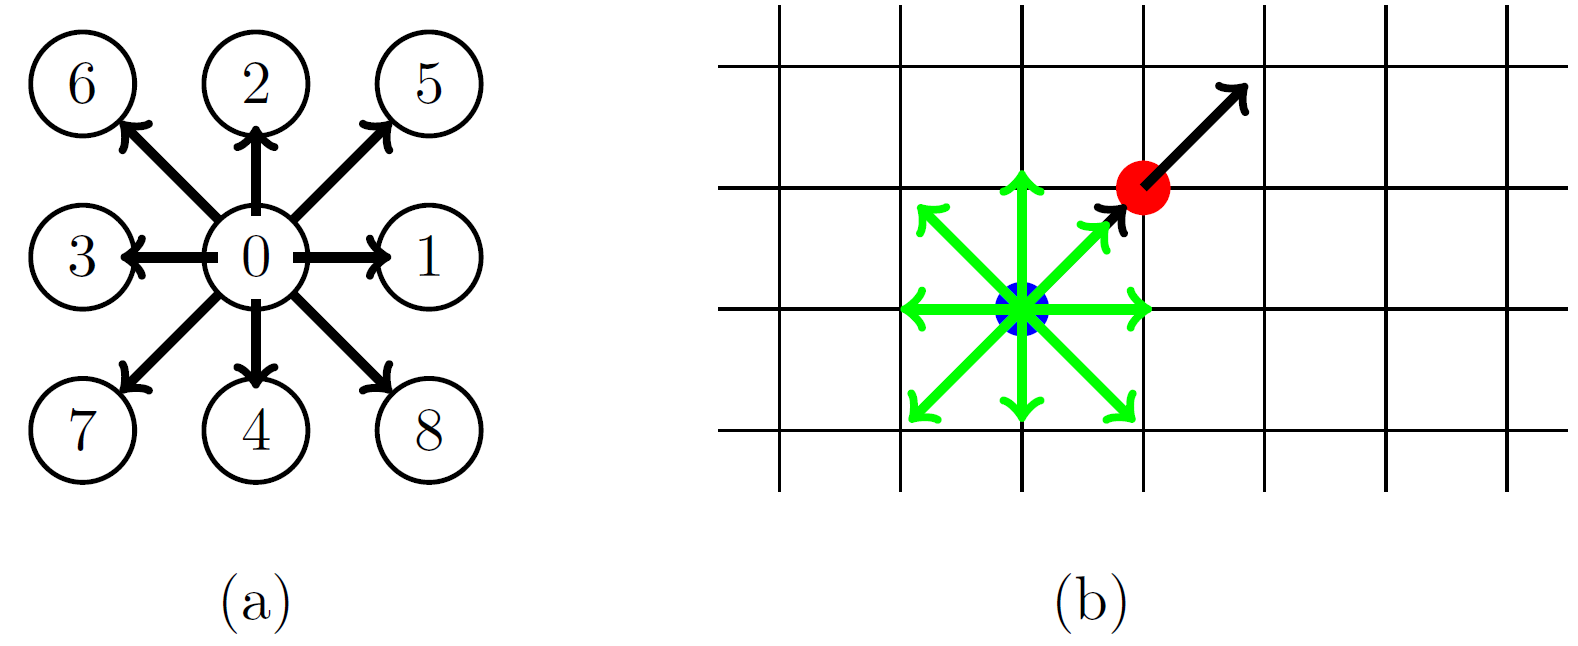
\includegraphics[width=10cm]{logos/Gitter_LBM.png}
   \caption{Discretization of \ac{bte}. (a) Discretization of the velocity space into nine discrete directions. The numbers $0,...,9$ uniquely identify the direction. (b) Spatial discretization for the two-dimensional lattice. The green arrows show the possible directions of the particle in the middle. For sake of simplicity, assume that the particle only moves in direction $5$. In the next time step the particle is located at the red dot.}
  \label{fig:mesh}
  \end{center}
\end{figure}

Finally, we get the discretized version of eq. \ref{eq-bte}:
\begin{equation}
\label{eq-discretizedBTE}
\underbrace{f_{i}(\mathbf{x}+\mathbf{c}_{i}\Delta t, t+\Delta t) - f_{i}(\mathbf{x})}_{streaming}
=\underbrace{-\omega(f_{i}(\mathbf{x})-f_{i}^{eq}(\mathbf{x},t))}_{collision},
\end{equation}
where the \textit{streaming} and \textit{collision process} are the key steps in the \ac{lbm} and $\omega=\frac{\Delta t}{\tau}$ is a relaxation parameter.

The equilibrium probability density function $f_{i}^{eq}$ can be computed as follows:
\begin{equation}
\label{eq-equilibrium}
f_{i}^{eq}=w_{i}\rho(x,t)(1+3\mathbf{c}_{i}\mathbf{u}(\mathbf{x},t)+\frac{9}{2}(\mathbf{c}_{i}\mathbf{u}(\mathbf{x},t))^{2}-\frac{3}{2}\mathbf{u}^{2}(\mathbf{x},t)),
\end{equation}
where $w_{i}=
\begin{cases}
\frac{4}{9}, ~if~i=0\\
\frac{1}{9}, ~if~i=1,2,3,4\\
\frac{1}{36}, ~if~i=5,6,7,8
\end{cases}$. Fig. \ref{fig:mesh}b gives a simplified example for eq. \ref{eq-discretizedBTE}.
\section{Moment update}\label{sec-momentUpdate}
In the \ac{lbm}, the density $\rho$ and velocity $\mathbf{u}$ are defined by the zeroth and first moments of the probability distribution function $f$, respectively:
\begin{align} 
\rho(\mathbf{x},t) &=  \int f(\mathbf{x}, \mathbf{u},t)~d^{3}\mathbf{u}, \\ 
\mathbf{u}(\mathbf{x},t) &=  \frac{1}{\rho(\mathbf{x})}\int f(\mathbf{x}, \mathbf{u},t)\cdot\mathbf{c}(\mathbf{u})~d^{3}\mathbf{u}.
\end{align}
The discretization of those equations yields
\begin{align}
\label{eq-density}
\rho(\mathbf{x}) &=  \sum\limits_{i} f_{i}, \\ 
\label{eq-velocity}
\mathbf{u}(\mathbf{x}) &=  \sum\limits_{i} f_{i}\mathbf{c}_{i}.
\end{align}
\section{Boundary conditions}\label{sec-boundaryConditions}
The boundary condition describes how the fluid flow behaves during streaming at the boundaries. We define the boundary node $\mathbf{x}_{b}$ to have at least one link to a solid or fluid node. 
Note, that the boundary conditions have to be placed in the correct step inside the \ac{lbm} (see code listing \ref{algo-pseudeocode}). For this reason we differentiate between the \textit{pre-streaming} probability density function $f_{i}^{\ast}$ and the \textit{post-streaming} probability density function $f_{i}$.
To apply boundary conditions the probability density function after the streaming $f_i$ is modified at each boundary node $\mathbf{x}_{b}$ given the pre-streaming probability density function $f_{i}^{\ast}$ in each time step:
\begin{equation}
f_i(\mathbf{x}_{b}+c_{i}\Delta t, t+\Delta t)=f_{i}^{\ast}(\mathbf{x}_b,t).
\end{equation}

One question that arises is where the boundary nodes $\mathbf{x}_b$ are defined. We distinguish between so called \textit{wet nodes} and \textit{dry nodes} due to different domains, i.e. computational and physical domain. In the former, the computation and physical domain is the same (i.e. the boundaries are placed on the lattice nodes) but this comes with a increased difficulty for the implementation. In the latter the physical domain is half a cell away from the computational domain (i.e. the boundaries are located between the lattice nodes) retaining second order accuracy as long as the boundary is placed exactly in the middle of the lattice nodes.

Below we describe several boundary conditions. One key advantage of the \ac{lbm} is its easy implementation of boundary conditions and in particular the arbitrary combination of boundary conditions as long as they do not contradict themselves.
\subsection*{Periodic boundary conditions}
For a periodic boundary condition the flow leaving a boundary re-enters the domain on the opposite side of the domain
\begin{equation}
f_{i}(\mathbf{x}_{1},t)=f_{i}(\mathbf{x}_{N},t),
\end{equation}
where $\mathbf{x}_{1}$ and $\mathbf{x}_{N}$ are the first and last node in the physical domain, respectively. Visually, we can imagine the bounce-back boundary conditions as if we have a cylindrical shape. Note, that therefore periodic boundary conditions conserve mass and momentum.
The periodic boundary condition is implicitly implemented by the streaming function.
\subsection*{Periodic boundary conditions with pressure variation}
The periodic boundary conditions with pressure variation add a density drop $\Delta\rho$ (or pressure drop $\Delta p$) between inlet and outlet. Note, that the pressure and density are related through the ideal gas of state $p=c_{s}^2\rho$, where $c_{s}$ is the speed of sound. \cite{CLAPEYRON.}
Let's assume that we want to model a pressure drop in x-direction, then it holds $\forall y\in\lbrace 1,...,l_{y}\rbrace$ that $p(x_{1},y,t)=p(x_{N},y,t)+\Delta\rho$, where $l_{y}$ denotes the diameter in y-direction and $x_1$ and $x_{N}$ denote the left-most and right-most node in the \ac{lbm}, respectively. Thus, we get $\rho_{out}=\frac{p_{out}}{c_{s}^2}$ and $\rho_{in}=\frac{p_{out}+\Delta p}{c_{s}^2}$, where the subscripts $in$ and $out$ denote the pressure values at the periodic boundaries.
Note, that the velocity is the same at the periodic boundaries: $\mathbf{u}(x_{1},y,t)=\mathbf{u}(x_{N},y,t)$.

Let's now assume virtual nodes $\mathbf{x}_{0}$ and $\mathbf{x}_{N+1}$ at both ends of the periodic boundaries. Note, that the virtual nodes $\mathbf{x}_{0}$ and $\mathbf{x}_{N}$ correspond to $\mathbf{x}_{N}$ and $\mathbf{x}_{1}$, respectively. Visually we can imagine this like (infinitely) many pipes connected to each other. We decompose the probability density function into a equilibrium part $f_{i}^{eq}$ and non-equilibrium part $f_{i}^{neq}$. The non-equilibrium probability density function is computed by $f_{i}^{neq}=f_{i}-f_{i}^{eq}$. Combining the correspondences of virtual nodes and nodes in the physical domain as well as the decomposition into (non)-equilibrium probability density function parts we obtain the inlet and outlet boundary condition, respectively
\begin{align}
f_{i}(x_0,y,t)&=f_{i}^{eq}(\rho_{in},\mathbf{u_N})+\underbrace{(f_{i}^{\ast}(x_N,y,t)-f_{i}^{eq}(x_N,y,t)}_{f_i^{neq}(x_N,y,t)}\rbrace\\
f_{i}(x_{N+1},y,t)&=f_{i}^{eq}(\rho_{out},\mathbf{u_1})+\underbrace{(f_{i}^{\ast}(x_1,y,t)-f_{i}^{eq}(x_1,y,t)}_{f_i^{neq}(x_1,y,t)}\rbrace
\end{align}
\subsection*{Bounce-back boundary}
The bounce-back boundary condition applies a no-slip condition at the boundary. It simulates the interaction between the fluid with a non-moving wall without slip. It can also be applied to a stationary obstacle such as a plate.
\begin{equation}
f_{\bar{i}}(\mathbf{x}_{b},t+\Delta t)=f_{i}^{\ast}(\mathbf{x}_{b},t),
\end{equation}
where the index $\bar{i}$ denotes the conjugate channel of $i$, e.g. the conjugate channel of $1$ is equal to $3$.
\subsection*{Moving wall}
The moving wall extends the bounce-back boundary condition by taking into account the gain or lose of momentum of particles during interaction with the moving wall. Thus, we extend the bounce-back boundary condition with an extra term for the momentum change
\begin{equation}
f_{\bar{i}}(\mathbf{x}_{b},t+\Delta t)=f_{i}^{\ast}(\mathbf{x}_{b},t)-2\omega_{i}\rho_{w}\frac{\mathbf{c}_{i}\cdot\mathbf{u}_{w}}{c_{s}^{2}},
\end{equation}
where $c_{s}$ is the speed of sound, $\rho_{w}$ and $\mathbf{u}_{w}$ are the density and velocity at the wall, respectively. The velocity at the wall $\mathbf{u}_{w}$ is equal to $\begin{pmatrix}U_{w}\\0\end{pmatrix}$ for a tangentially moving wall in x-direction with wall velocity $U_{w}$.  
There are two main options for the estimation of the density at the wall $\rho_{w}$:
\begin{enumerate}
\item The density at the wall $\rho_{w}$ is equal to the \textit{average} density $\bar{\rho}$.
\item The density at the wall $\rho_{w}$ is \textit{extrapolated} from the densities $\rho$ next to the wall. Depending on the order of the extrapolation, we use more or less nodes.
\end{enumerate}
\subsection*{Open boundary}
\cite{Kruger.2016} describe open boundaries consist of inlets and outlets where the flow can either enter or leave the computation domain and where we typically \textit{impose velocity or density profiles}. We implement the inlet as follows:
\begin{equation}
f_{i}(\mathbf{x}_{b},t+\Delta t)=f_{i}^{eq}(\rho_{in},\mathbf{u}_{in})~\forall i\in\lbrace 0,...,8\rbrace,
\end{equation}
where $\rho_{in}$ and $\mathbf{u}_{in}$ are the density and velocity at the inlet, respectively.

For the outlet, we implement a first-order extrapolation scheme by using the information from the second last node $\mathbf{x}_{b_{2}}=\mathbf{x}_{b}-\Delta\mathbf{x}$
\begin{equation}
f_{i}(\mathbf{x}_{b},t+\Delta t)=f_{i}(\mathbf{x}_{b_{2}},t),
\end{equation}
where $i$ denotes the indices pointing into the domain.
\chapter{Implementation}\label{ch-implementation}
In this chapter we will describe how we implement the algorithm using \textit{Python} as programming language.
\section{Overview}
Code listing \ref{algo-pseudeocode} shows the pseudocode of the iteration loop of the \ac{lbm}. As input we can specify the geometry of the physical domain, the boundary conditions (see section \ref{sec-boundaryConditions} for more details) as well as the initial conditions. 

First we initialize the density $\rho$ and velocity $\mathbf{u}$ and compute the initial value of the probability density function $f_{i}^{eq}=f_{i}$. 

Then we iterate in a loop over several steps as long as the stopping criterion (e.g. maximum time steps) is not satisfied. Note, that there is some flexibility when to apply which step. \cite{Kruger.2016, Succi.2018} The following order of steps corresponds to the order in the implementation of the \ac{lbm}. We first compute the equilibrium function $f_{i}^{eq}$ given the current density $\rho$ and velocity $\mathbf{u}$. In the collision step we simulate the effects of collisions between particles (see section \ref{sec-bte} for more details). After that, we simulate the streaming of $f_i$, i.e. we simulate the movement of particles to the nearest neighbour lattice nodes using the D2Q9 discretization. Then we apply potential boundary conditions on the probability density function $f_i$. Note, that we first apply the streaming operation at every node (including the boundary nodes $\mathbf{x}_{b}$) and then correct the boundary nodes $\mathbf{x}_{f}$ after the streaming. This has the advantage that the implementation of the streaming is easier. Lastly, we compute the density $\rho$ and velocity $\mathbf{u}$ (see section \ref{sec-momentUpdate} for details on the formulas on how to compute the macroscopic quantities).

After running the \ac{lbm} we can obtain the density $\rho$ and velocity $\mathbf{u}$ as macroscopic quantities.

\begin{algorithm}
 \caption{\label{algo-pseudeocode}Pseudocode of the iteration loop of the \ac{lbm}.}
     \SetAlgoLined
     \KwInput{Geometry and parameters $l$, $h$, $U$, $\nu$,...; boundary conditions; initial conditions}
     \KwOutput{Final density $\rho$ and velocity $\mathbf{u}$}
     initialize $\rho$ and $\mathbf{u}$ \\
     compute $f_i$ and $f_i^{eq}$ \\
     \While{stopping criterion is not satisfied}{
      compute equilibrium function $\rho,~\mathbf{u}\rightarrow f_{i}^{eq}$\Comment*[f]{eq. \ref{eq-equilibrium}}\\
      collision step $f_{i}^{\ast}=f_{i}(\mathbf{x},t)-\frac{\Delta t}{\tau}(f_{i}(\mathbf{x},t)-f_{i}^{eq}(\mathbf{x},t))$ \Comment*[f]{eq. \ref{eq-discretizedBTE}}\\
      streaming $f_{i}(\mathbf{x}+c_{i}\Delta t, t+\Delta t)=f_{i}^{\ast}(\mathbf{x},t)$ \Comment*[f]{eq. \ref{eq-discretizedBTE}}\\
      apply boundary conditions $f_i(\mathbf{x}_{b}+c_{i}\Delta t, t+\Delta t)=f_{i}^{\ast}(\mathbf{x}_b,t)$ \Comment*[f]{section \ref{sec-boundaryConditions}}\\
      moment update $f_i \rightarrow \rho,~\mathbf{u}$ \Comment*[f]{eq. \ref{eq-density} \& \ref{eq-velocity}}
     }
\end{algorithm}
\section{Basic implementation in Python}
In this section we show how we implemented the basic equations and data structures introduced in chapter \ref{ch-method}. We use Python as programming language and use the python libraries \textit{numpy} \cite{Oliphant.2006,vanderWalt.2011} for array operations, \textit{scipy} \cite{Virtanen.2020} for some more complex scientific computations and \textit{matplotlib} \cite{Hunter.2007} for visualizing the obtained results. And key advantage of numpy is to vectorize arrays, which lowers the computational time.

We represent the (discrete) probability density function $f_{i}(\mathbf{x})$ as a numpy array of size $l_{x}\times l_{y}\times 9$, where $l_{x}$ and $l_{y}$ are the size of the lattice in x- and y-direction, respectively. The last dimension (e.g. $9$) of the numpy array corresponds to the discretized velocity direction.
We represent the velocity directions $\mathbf{c}$ and the weights $w_{i}$ as numpy arrays with size $9\times 2$ and $9$, respectively.

In steps 4 and 5 of code listing \ref{algo-pseudeocode} we simulate the collision part of eq. \ref{eq-discretizedBTE}. We implement the computation of the equilibrium probability density function $f_{i}^{eq}$ of eq. \ref{eq-equilibrium} and the right-hand side of eq. \ref{eq-discretizedBTE} with vectorized numpy code. 

Code listing \ref{algo-collision} shows the implementation of the collision step, separated into equilibrium probability density function computation and the collision.
\begin{algorithm}
 \caption{\label{algo-collision}Python implementation of the collision step. Note that the symbol $@$ is a shorthand for the matrix multiplication in NumPy.}
     \SetAlgoLined
     \KwInput{density $\rho$; velocity $\mathbf{u}$, relaxation parameter omega $\omega$}
     \KwOutput{Probability density function before streaming $f_{i}^{\ast}$}
     w\textunderscore i = np.array([4/9, 1/9, 1/9, 1/9, 1/9, 1/36, 1/36, 1/36, 1/36])\\
     \SetKwFunction{FEq}{f\textunderscore eq}
\Fn{\FEq{rho:np.ndarray, u:np.ndarray}$\rightarrow$np.ndarray}{
w\textunderscore i = w\textunderscore i[np.newaxis, np.newaxis, ...]\\
		ci\textunderscore u = u @ c\textunderscore i.T\\
		uu = (np.linalg.norm(u, axis=-1) ** 2)[..., np.newaxis]\\
		rho = rho[..., np.newaxis]\\
        \KwRet w\textunderscore i * rho * 
        (1 +
            3 * ci\textunderscore u +
            9/2 * ci\textunderscore u ** 2 -
            3/2 * uu)
  }
  f\textunderscore pre = f + (f\textunderscore eq(rho, u) - f) * omega
\end{algorithm}

In steps 6 of code listing \ref{algo-pseudeocode} we simulate the streaming part of eq. \ref{eq-discretizedBTE}. Code listing \ref{algo-streaming} shows the implementation using \textit{np.roll}.  The function rolls the the data in the direction specified by the \textit{axis} argument. With the argument $shift$ we specify the number of places elements are shifted according to the discrete velocity directions $\mathbf{c}$. Note, that the function automatically implements the periodic boundary condition.
\begin{algorithm}
 \caption{\label{algo-streaming}Python implementation of the streaming step.}
     \SetAlgoLined
     \KwInput{Probability density function before streaming $f_{i}^{\ast}$}
     \KwOutput{Probability density function after streaming $f_{i}$}
     c\textunderscore i = np.array([[0,0],[1,0],[0,1],[-1,0],[0,-1],[1,1],[-1,1],[-1,-1],[1,-1]])\\
     \SetKwFunction{FStream}{streaming}
\Fn{\FStream{f\textunderscore pre:np.ndarray}$\rightarrow$np.ndarray}{
f\textunderscore post = np.zeros\textunderscore like(f\textunderscore pre)\\
\For{$i$ \KwTo\Range $(9)$}{
f\textunderscore post[..., i]=np.roll(f\textunderscore pre[...,i], shift=c\textunderscore i[i], axis=(0,1))
}
\KwRet f\textunderscore post
}
\end{algorithm}

For the other boundary conditions we implement additional functions which correct the boundary nodes as described in section \ref{sec-boundaryConditions}. Code listing \ref{algo-boundaryConditions} gives an overview of the different implementations.
The implementation of the boundary conditions follows directly from the formulas. For example when we implement the bounce-back boundary condition on a non-moving wall at the bottom, we bounce back channels $4$, $7$ and $8$. That is, we assign the pre-streaming probability density function at the boundary nodes $f_{i}^{\ast}(\mathbf{x}_{b},t)$ to the conjugate channels (e.g. $2$, $5$, $6$) of the post-streaming probability density function at the boundary nodes $f_{i}(\mathbf{x}_{b},t+\Delta t)$. 
For the implementation of the bounce-back condition for a object inside the domain such as a vertical plate we apply the bounce-back conditions on the corresponding two columns. We have to take corner nodes into special consideration. There we just bounce-back two channels. For example consider the lattice node at the top corner on the left side of the plate. There we only bounce back channels $1$ and $8$.
We implement the moving wall boundary condition in a similar way but with the additional term $-2\omega_{i}\rho_{w}\frac{\mathbf{c}_{i}\cdot \mathbf{u}_{w}}{c_{s}^{2}}$ to take the momentum change into account. For the density at the wall $\rho_{w}$ we use the average density.
For the inlet boundary condition we assign the equilibrium probability density function given the inlet density $\rho_{in}$ and inlet velocity $\mathbf{u}_{in}$. 
For the outlet boundary condition we assign the second last nodes of the probability density function of the previous time step to the last nodes of the probability density function of the current time step.
For the periodic boundary conditions with pressure variation we extend the domain with virtual nodes at both ends of the periodic boundaries. The implementation then is straightforward. 
\begin{algorithm}
 \caption{\label{algo-boundaryConditions}Exemplar Python implementation of the boundary condition. Note that the index i refers to specific channels depending on the boundary conditions. For details see section \ref{sec-boundaryConditions}. Note that $@$ and $.T$ are shorthands for matrix multiplication and transpose in NumPy.}
     \SetAlgoLined
     \# Bounce-back\\
     f\textunderscore post[$\mathbf{x}$\textunderscore b, conjugate[i]]=f\textunderscore pre[$\mathbf{x}$\textunderscore b,i] \\
     \# Moving wall\\
          f\textunderscore post[$\mathbf{x}$\textunderscore b, conjugate[i]]=f\textunderscore pre[$\mathbf{x}$\textunderscore b,i] - 2$\cdot$ w\textunderscore i[i]$\cdot$ avg\textunderscore rho $\cdot$ (c\textunderscore i[i] @ u\textunderscore w) /(c\textunderscore s **2) \\
          \# Inlet\\
     f\textunderscore post[0,:, i]=f\textunderscore eq(rho\textunderscore in,u\textunderscore in)[0,:,i]\\
     \# Outlet\\
     f\textunderscore post[-1,:, i]=f\textunderscore previous[-2,:,i]\\
     \# Periodic boundary condition with pressure variation\\
  f\textunderscore post[0,:,i]=f\textunderscore eq(rho\textunderscore in, u[-2,...])[...,i].T + (f\textunderscore pre[-2,:,i]-f\textunderscore eq(rho, u)[-2,:,i])
\end{algorithm}
\section{Parallelization}\label{sec-parallelization}
We parallelize the \ac{lbm} using spatial domain decomposition and \acf{mpi} \cite{Dalcin.2005, Dalcin.2008, Dalcin.2011}. \ac{mpi} is a \textit{communication protocol} for programming parallel computers, i.e. \ac{simd} \cite{Flynn.1972} by executing the same operation on multiple data points simultaneously.

We decompose the computational domain into sub domain using a cartesian topology. To implement this we use the \ac{mpi} function \textsf{Create\textunderscore cart} creating a cartesian topology.
We decompose the full computational domain into sub domains of roughly equal size (see fig. \ref{fig:parallelizationScheme} for an example).
If the domain is not exactly divisible into the subdomains we extend the rightmost or topmost process with the division remainder. Note that this could lead to imbalanced subdomains, but comes with an easier transformation from global coordinates into local (i.e. process-level) coordinates. For the communication we extend the sub domains with ghost cells around the actual computational domain.

The collision step of the \ac{lbm} is embarrassingly parallel, since the collision step operates only locally and thus requires no communication between processes.

For the streaming step we have to consider particles moving from one domain to a neighboring domain (i.e. another process) corresponding the the channel. We implement this by extending each domain by \textit{ghost cells} around the actual computational domain. Before streaming we communicate the lattice nodes adjacent to the ghost region into the ghost points of the neighboring domain according to the specific channel. 

\begin{figure}
  \begin{center}
   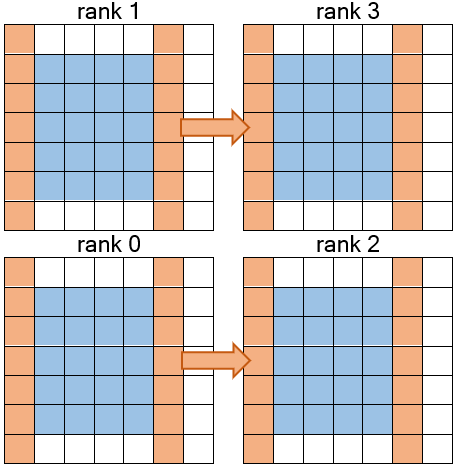
\includegraphics[width=10cm]{../figures/parallelization_strategy/parallelization_scheme.png}
   \caption{Example of spatial domain decomposition and communication strategy. We decompose the original domain into a $2\times 2$ grid of sub domains of roughly equal size (blue lattice points). We add additional ghost nodes around the actual computational domain (white lattice points). In the communication step, we communicate the rightmost, leftmost, bottommost and topmost lattice points in the actual computational domain into the neighboring ghost lattice points. In the figure we show the communication step of the rightmost lattice points to the ghost cells of the respective  right neighbors.}
  \label{fig:parallelizationScheme}
  \end{center}
\end{figure}
Let's consider the example of fig. \ref{fig:parallelizationScheme}. We consider a $2\times 2$ decomposition of the original computational domain and we denote the lower left subdomain with rank $0$, upper left with rank $1$, lower right with rank $2$ and upper right with rank $3$. W.l.o.g., we first consider the rightmost nodes $\mathbf{x}_r$ of each sub domain. We communicate the rightmost nodes $\mathbf{x}_r$ from each process to the neighboring process on the right. In our particular example this means that we communicate the rightmost nodes $\mathbf{x}_r$ of the process with rank $0$ to the ghost cells on the left side of process with rank $2$. Accordingly, we communicate from process $1$ to process $3$. Note that we do not communicate from process $2$ to $0$ or $3$ to $1$ or more generally we do not communicate outer boundaries of edge domains, since we set \textsf{periods=(False, False)} when calling the \ac{mpi} function \textsf{Create\textunderscore cart}. This slightly reduces the amount of required communication.
We repeat this procedure for the leftmost nodes $\mathbf{x}_l$, bottommost nodes $\mathbf{x}_b$ and topmost nodes $\mathbf{x}_t$ accordingly. This totals in four communication steps. Code listing \ref{algo-communication} shows the implementation of the communication step. We call the communication step right before the streaming step in code listing \ref{algo-pseudeocode}.
\begin{algorithm}
 \caption{\label{algo-communication}Python implementation of the communication step.}
     \SetAlgoLined
     \SetKwFunction{OuterComm}{communication}
\textbf{from} mpi4py \textbf{import} MPI\\
\textbf{from} typing \textbf{import} Callable\\
\Fn{\OuterComm{comm: MPI.Intracomm}$\rightarrow$Callable[[np.ndarray], np.ndarray]}{
    left\textunderscore src, left\textunderscore dst = comm.Shift(direction=0, disp=-1)\\
    right\textunderscore src, right\textunderscore dst = comm.Shift(direction=0, disp=1)\\
    bottom\textunderscore src, bottom\textunderscore dst = comm.Shift(direction=1, disp=-1)\\
    top\textunderscore src, top\textunderscore dst = comm.Shift(direction=1, disp=1)\\
    
    	\SetKwFunction{InnerComm}{communicate}
	\Fn{\InnerComm{f: np.ndarray}$\rightarrow$np.ndarray}{
	        \# send to left\\
        recvbuf = f[-1, ...].copy()\\
        comm.Sendrecv(f[1, ...].copy(), left\textunderscore dst, recvbuf=recvbuf, source=left\textunderscore src)\\
        f[-1, ...] = recvbuf\\
        \# send to right\\
        recvbuf = f[0, ...].copy()\\
        comm.Sendrecv(f[-2, ...].copy(), right\textunderscore dst, recvbuf=recvbuf, source=right\textunderscore src)\\
        f[0, ...] = recvbuf\\
        \# send to bottom\\
        recvbuf = f[:, -1, :].copy()\\
        comm.Sendrecv(f[:, 1, :].copy(), bottom\textunderscore dst, recvbuf=recvbuf, source=bottom\textunderscore src)\\
        f[:, -1, :] = recvbuf\\
        \# send to top\\
        recvbuf = f[:, 0, :].copy()\\
        comm.Sendrecv(f[:, -2, :].copy(), top\textunderscore dst, recvbuf=recvbuf, source=top\textunderscore src)\\
        f[:, 0, :] = recvbuf\\
        \KwRet f

}
    \KwRet \InnerComm
    }

\end{algorithm}

In the boundary conditions we transform global coordinates $global\textunderscore coord$ into local (i.e. process-level) coordinates $local\textunderscore coord$ in order to apply the boundary conditions at the correct global position in the lattice grid. Since we only increase the size of sub domains on the right or top, we can compute local coordinates straightforward. From the \ac{mpi} function \textsf{Get\textunderscore coords} we get the process coordinates $proc\textunderscore coord$ of the cartesian topology. We compute the local $x$ coordinate $local\textunderscore coord_{x}$ as follows:
\begin{equation}
local\textunderscore coord_{x}=global\textunderscore coord_{x}-proc\textunderscore coord_{x}*(l_{x}//proc\textunderscore size_{x}) +1,
\end{equation}
where $l_{x}$ is the lattice grid size in $x$ direction and $//$ denotes the integer division. Note, that we add $1$, since we have to take the ghost cell in the specific process into account. We can apply computation similarly for the local $x$ coordinate $local\textunderscore coord_{y}$.
\section{Software quality}
\subsection*{Static typing}
Python is a dynamically typed language. That is that the Python interpreter does type checking only in runtime and the type of a variable is allowed to change. The opposite of dynamic typing is static typing. It is introduced by \textit{PEP 484}\footnote{\url{https://www.python.org/dev/peps/pep-0484/}} in Python. In static typing, the types of the variables are checked before runtime and the change of types is generally not allowed. Note, as an exception type casting is a way to change the type of a variable in many languages.

Dynamic typing allows for rapid prototyping and thus it enables fast software development. On the other side static typing can help to catch errors due to type errors, document the code and help to build a cleaner software architecture. The last point in particular ensures that the programmer thinks about the types of the variables and uses the correct types. Thus, in any larger project typing is critical to build and maintain clean code.
\subsection*{Unit testing}
One key component of every software project is extensive testing of the software. To this end, we implement several unit tests in order to validate the expected behavior of the implemented functions. 
More specifically, we test the computation of the density and velocity, the streaming function, mass preservation (i.e. first and second mass conservation equation and first and second impulse conservation equation from the Navier-Stokes Equations as well as a long run mass conservation test over $10000$ time steps) and the boundary conditions.
Additionally, we validate the parallelized implementation by comparing it to the serial implementation of the von K\'{a}rm\'{a}n's vortex street over $400$ time steps using different number of nodes. 

We integrate the unit tests into \ac{ci} using \textit{Travis CI} as build server so that the implementation and its potential unintentional modifications are validated for each commit to the repository.
\chapter{Numerical results}\label{ch-results}
To demonstrate the \ac{lbm} implementation we conduct several experiments with different combinations of boundary conditions. First we consider a \textit{shear wave decay} (section \ref{sec-shearWave}) to validate whether our implementation preserves mass as well as to show how $\omega$ relates to the kinematic viscosity $\nu$. In sections \ref{sec-couette} and \ref{sec-pouseuille} we implement well known laminar flows, i.e. \textit{couette} and \textit{pouiseuille} flow, from the literature and compare it to their analytical solutions, respectively. In section \ref{sec-karman} we implement the \textit{von K\'{a}rm\'{a}n's vortex street} and in the following section \ref{sec-scaling} how we can reduce computational complexity by spatial domain decomposition as introduced in section \ref{sec-parallelization}.
\section{Shear wave decay}\label{sec-shearWave}
The shear wave decay simulates a physical domain with only periodic boundary conditions which is in a initial state and its incremental steps towards the equilibrium state. One common practical and illustrative application of it, is the simulation of the breaking of a water dam. This exemplar application also shows the importance of simulations as the \ac{lbm} to simulate rather than applying it in a real-world setting potentially causing mass destruction and high costs.

We choose the following simulation parameters for our experiments:
\begin{itemize}
\setlength\itemsep{0.15em}
\item lattice grid shape $=50\times 50$
\item $\omega=1.0$
\item Sinusoidal density in x-direction $\rho(\mathbf{x},0)=\rho_{0}+\epsilon_{\rho}\sin(\frac{2\pi x}{l_x})$
\begin{itemize}
\setlength\itemsep{0.1em}
\item $\rho_{0}(\mathbf{x})=0.5$
\item $\epsilon_{\rho}=0.08$
\item $\mathbf{u}_{initial}(\mathbf{x})=0.0$
\end{itemize}
\item Sinusoidal velocity in y-direction $\mathbf{u}_{x}(\mathbf{x},0)=\epsilon_{\mathbf{u}}\sin(\frac{2\pi y}{l_y})$
\begin{itemize}
\setlength\itemsep{0.1em}
\item $\rho_{initial}(\mathbf{x})=0.0$
\item $\epsilon_{\mathbf{u}}=0.08$
\end{itemize}
\item time steps $=2000$
\end{itemize}
\section{Planar couette flow}\label{sec-couette}
The planar couette flow is a steady, laminar flow between two infinitely long, parallel plates with a fixed distance. One of those plates moves tangentially at a velocity of $U$ relative to the other plate, which itself is stationary. The flow is caused by the viscous drag force acting on the fluid.

We choose the following simulation parameters for our experiments about the planar couette flow:
\begin{itemize}
\setlength\itemsep{0.15em}
\item lattice grid shape $=20\times 30$
\item $\omega=1.0$
\item $U=0.05$
\item $\rho_{initial}(\mathbf{x})=1.0$
\item $\mathbf{u}_{initial}(\mathbf{x})=0.0$
\item time steps $=4000$
\end{itemize}

We can see that the simulated solution almost exactly reproduces the analytical solution. This shows that the bounce-back boundary condition is first-order accurate. Furthermore, it is also second-order accurate, since the boundary values and its first-order derivative are reproduced exactly.

%TODO write plotting for this
We can also observe that the solution is viscosity-independent.
\section{Planar poiseuille flow}\label{sec-pouseuille}
The planar poiseuille flow is a steady flow between two non-moving plates. The flow is caused by a constant pressure gradient $\frac{dp}{dx}$ in the axial direction, $x$, parallel to two infinitely long parallel plates, seperated by a distance $h$.

We choose the following simulation parameters for our experiments about the planar poiseuille flow:
\begin{itemize}
\setlength\itemsep{0.15em}
\item lattice grid shape $=200\times 30$
\item $\omega=1.5$
\item $p_{out}=\frac{1}{3}$
\item $\Delta p=0.001111$
\item $\rho_{initial}(\mathbf{x})=1.0$
\item $\mathbf{u}_{initial}(\mathbf{x})=0.0$
\item time steps $=5000$
\end{itemize}

Some error can occur due to:
\begin{itemize}
\item Inaccuracy introduced by the bounce-back boundary condition. In particular, the error depends on the viscosity.\cite{Kruger.2016}
\end{itemize}

%TODO write plot for viscosity test
In fig. xyz we can observe that the boundary velocity changes for different $\omega 's$. This in turn shows that the poiseuille flow simulation is viscosity-dependent. This is called \textit{numerical boundary slip}. \cite{Kruger.2016}
\section{Von K\'{a}rm\'{a}n's vortex street}\label{sec-karman}
\section{Scaling tests}\label{sec-scaling}
\chapter{Conclusions}\label{ch-conclusion}
In this report we described the \ac{lbm} and its implementation in Python. We also show several applications of the \ac{lbm} to specific problems and compare the simulation results to analytical solutions if possible. We extend the serial implementation by using spatial domain decomposition to reduce computational costs by means of parallelization.

In chapter \ref{ch-method} we describe the theoretical foundations of the \ac{lbm}. Starting from the continuous \ac{bte} we show how to discretize the \ac{bte} to obtain the \ac{lbm}.

In chapter \ref{ch-implementation} we discussed the implementation and more specifically the parallelization of the \ac{lbm}. We demonstrate by using the high-level language Python that implementations of the discrete equations are straightforward. We show how to reduce the computational burden by decompose the domain spatially into subdomains. Note, that the collision step is embarrassingly parallel. For the streaming step we use ghost cells to communicate adjacent lattice nodes to neighboring process. For the boundary conditions we transform global indices into local indicies in order to apply boundary conditions on the correct boundary nodes.

In chapter \ref{ch-results} we demonstrate in several applications the correctness of our \ac{lbm} implementation by comparing the simulation results to analytical solutions from the literature. In addition, we demonstrate the speed-up that we can obtain from the spatial domain decomposition parallelization strategy of the \ac{lbm} for the von K\'{a}rm\'{a}n's vortex street.

\newpage

\bibliographystyle{unsrt}
\bibliography{biblio}

\end{document}
